\section{Implementation}
\label{sec:implementation}

To showcase and benchmark my work, I created an Android App that visualizes sensor data from the device that it runs on and also from connected Android Wear devices.
The app is called Sensor Data Logger (\ref{fig:sensorDataLoggerApp}) and can be downloaded for free from the Google Play Store\footnote{\href{https://play.google.com/store/apps/details?id=net.steppschuh.sensordatalogger}{https://play.google.com/store/apps/details?id=net.steppschuh.sensordatalogger}}.

\begin{figure}[H]
	\href{https://github.com/Steppschuh/Sensor-Data-Logger}{
		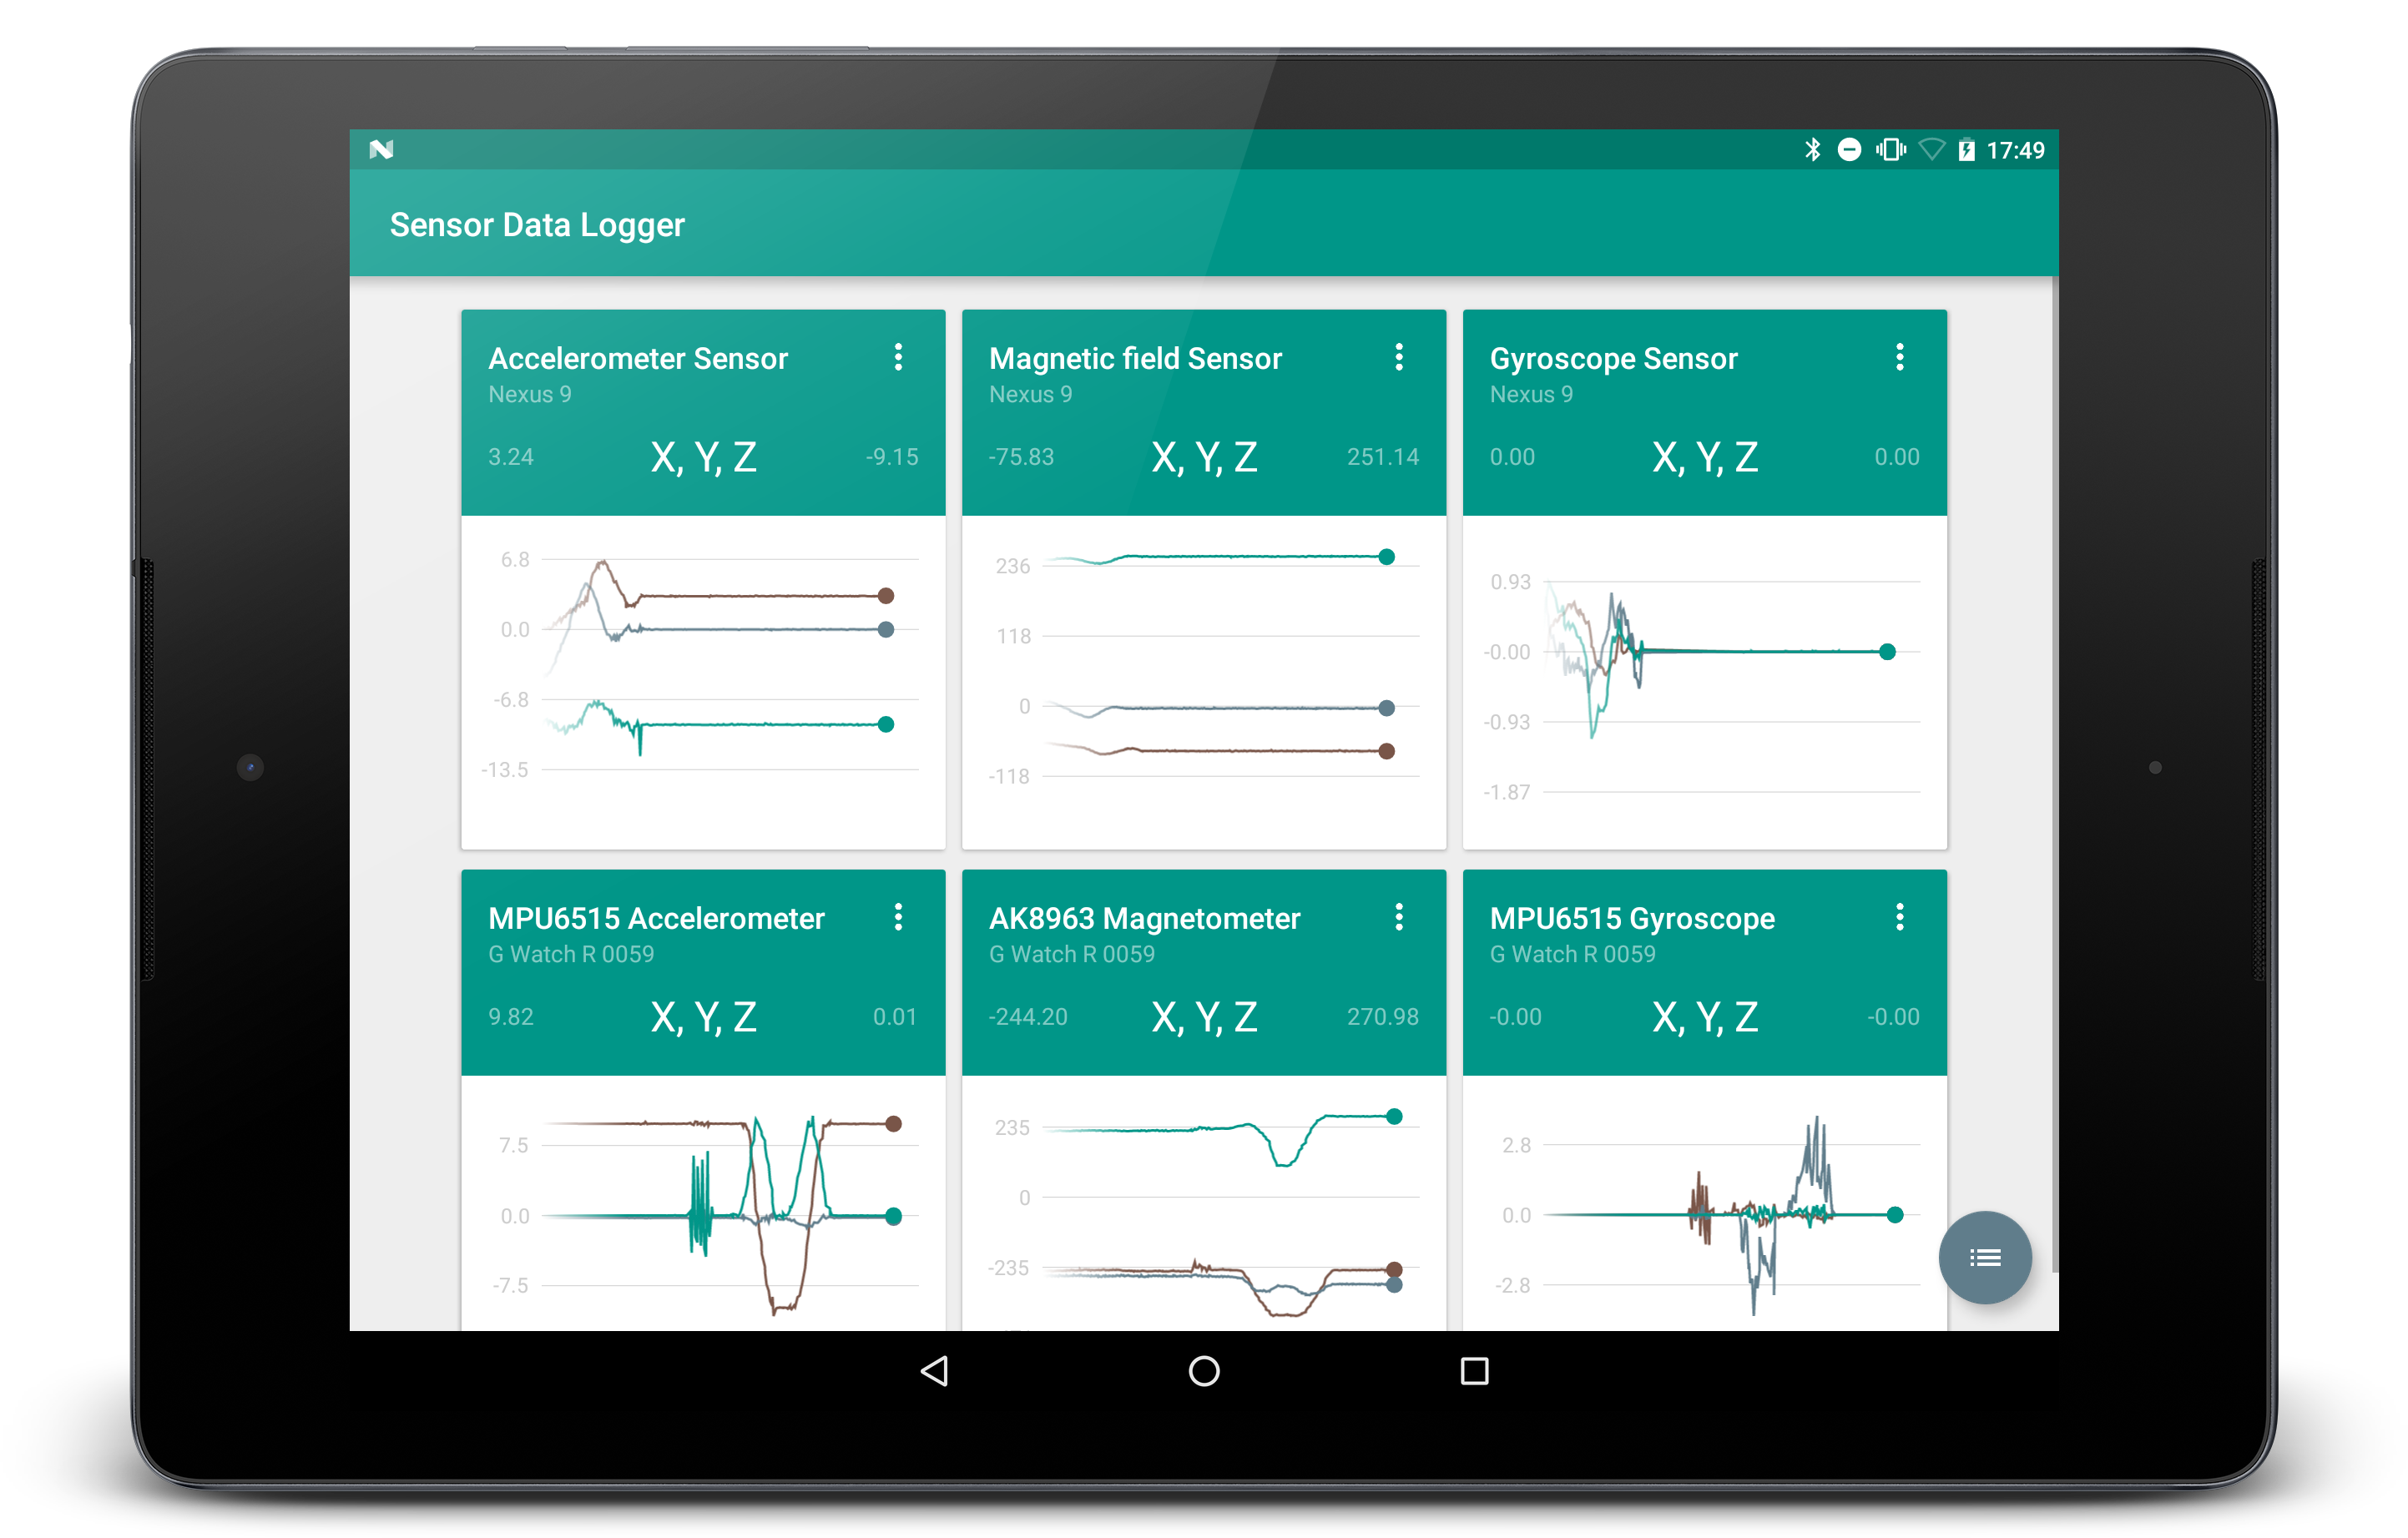
\includegraphics[width=\linewidth]{images/app/charts_landscape_framed.png}
	}
	\caption[Caption for Sensor Data Logger App]{Sensor Data Logger App}
	\label{fig:sensorDataLoggerApp}
\end{figure}

Code samples in the following sections are snippets from this project and can be seen in context in the GitHub repository\footnote{\href{https://github.com/Steppschuh/Sensor-Data-Logger}{https://github.com/Steppschuh/Sensor-Data-Logger}}.

\clearpage

\subsection{Accessing Data}
\begin{itemize}[noitemsep]
	\item The Android sensor manager
	\item Registereing sensor event listeners
	\item Collectiong sensor event data
\end{itemize}
\lipsum[1]
\lipsum[2]
\lipsum[3]
\lipsum[4]
\lipsum[5]
\lipsum[1]
\lipsum[2]
\lipsum[3]
\lipsum[4]
\lipsum[5]

\subsection{Transferring Data}
\begin{itemize}[noitemsep]
	\item What to transfer
		\begin{itemize}
			\item suitable data types
			\item serialization
		\end{itemize}
	\item How to transfer
		\begin{itemize}
			\item Available APIs and Protocols
			\item Pros and cons of different methods
		\end{itemize}
\end{itemize}
\lipsum[1]
\lipsum[2]
\lipsum[3]
\lipsum[4]
\lipsum[5]
\lipsum[1]
\lipsum[2]
\lipsum[3]
\lipsum[4]
\lipsum[5]
\lipsum[2]
\lipsum[3]
\lipsum[4]
\lipsum[5]


\clearpage